% Printed 282; principal PDF 289; Google PDF 293.
\par\clearpage
\noindent\makebox[0pt][l]{\fontsize{13}{16}\selectfont 282}\hfill{\small\textbf{BRIEFWECHSEL.}}\hfill\null\par\medskip

\noindent ders angeben können, worüber Sie eine Erläuterung wünschen. Diesmal bemerke ich nur, dass bei dieser Aufstellung zwei Hauptschritte nötig sind.

I.\quad Aufstellung einer Tabelle, die sich \textls[120]{bloß} aus den Messungen am Ort ergibt und daher noch nicht orientiert ist.

II.\quad Orientierung der Tabelle durch Hinzufügen einer Konstanten. Dabei bemerke ich, dass ich die erste Tabelle der Bequemlichkeit halber gern so einrichte, dass sie schon sehr nahe an der richtigen Orientierung liegt.

In die erste Tabelle braucht man nur diejenigen Richtungen einzutragen, die auf Winkelmessungen beruhen, die einander in irgendeiner Weise kontrollieren, und von den übrigen nur diejenigen, die für die absolute Orientierung nötig sein können. Im vorliegenden Fall sind erstere [die Richtungen]
\[
\GaussRightBrace{
\begin{array}{@{}r@{\enspace}l@{}}
 1&\text{Neuenfelde}\\
 2&\text{Altenwerder}\\
 3&\text{Altona, Heliotrop}\\
 4&\text{Hamburg}\\
 5&\text{Wilhelmsburg}
\end{array}
}\quad\odot
\]
und letztere [die Richtungen nach] dem Pfahl, dem Meridianpfahl und etwa nach Rönneberg. Ich hätte unter letzteren auch Harburg aufgenommen, wenn es mit Repetition eingeschnitten worden wäre.

Sämtliche Messungen, die sich auf die Punkte \(\odot\) beziehen, sind folgende*)
\[
\GaussRightBrace{
\begin{array}{@{}r@{\quad}r@{\qquad}r@{\;}r@{\;}r@{}}
 1.2&5&41^\circ&4'&39''{,}700\\
 1.3&4&45&11&31{,}400\\
 1.4&4&54&45&31{,}562\\
 1.5&5&85&36&40{,}200\\
 2.3&1&4&6&50{,}750\\
 2.5&10&44&32&2{,}275\\
 3.4&28&9&34&1{,}973\\
 3.5&2&40&25&10{,}000\\
 4.5&20&30&51&9{,}255
\end{array}
}\quad\mathrm{A}
\]

\par\smallskip\noindent\rule{4cm}{.4pt}\par
{\footnotesize\noindent\hspace*{\parindent}*) Ich habe die Mittel zum Teil etwas anders genommen als Herr \textsc{Peters}.\par}

% Printed 283; principal PDF 290; Google PDF 294.
\par\clearpage
\noindent\null\hfill{\small\textbf{STATIONSAUSGLEICHUNGEN.}}\hfill\makebox[0pt][r]{\fontsize{13}{16}\selectfont 283}\par\medskip

Um Tabelle I für die Punkte \(\odot\) zu erhalten, muss zunächst eine andere, angenäherte Tabelle vorausgehen, in der die Messungen A \textls[120]{noch nicht} ausgeglichen sind. Damit sie wenigstens ungefähr orientiert ist, bemerke ich, dass meine frühere Tabelle für Altona Folgendes enthält.
\[
\begin{array}{@{}l@{\;}r@{\;}r@{\;}l@{}}
 \text{\hbox to 8.7em{Harburg\hfil.\hfil.\hfil.\hfil.\hfil.\hfil.\hfil.\hfil.\hfil.}}&344^\circ&52'&54''{,}294\\
 \text{\hbox to 8.7em{Meridianpfahl\hfil.\hfil.\hfil.\hfil.}}&359&59&56{,}741.
\end{array}
\]

Für Vahrendorf ergibt sich damit Folgendes.
\[
\begin{array}{@{}l@{\quad}r@{\quad}l@{}}
 \text{aus Harburg}&
 \GaussOldenburgLeftBrace{\begin{array}{@{}r@{\;}r@{\;}r@{}}344^\circ&52'&54''{,}294\\28&41&26{,}413\end{array}}&\\[3.5pt]
 \cline{2-2}
 &13\quad34\quad20{,}707&
 \begin{array}[t]{@{}c@{}}\text{15 Beob., denen ich nur halbes}\\\text{Gewicht beilege.}\end{array}\\[5pt]
 \text{aus Meridianpfahl}&
 \GaussOldenburgLeftBrace{\begin{array}{@{}r@{\;}r@{\;}r@{}}359&59&56{,}741\\13&34&23{,}400\end{array}}&\\[3.5pt]
 \cline{2-2}
 &13\quad34\quad20{,}141&\text{43 Beob.}\\
 \cline{2-2}
 &13^\circ\;34'\;20''{,}225&\text{Mittel.}
\end{array}
\]

Vom Vahrendorfer \textls[120]{Pfahl} aus wäre das Azimut von Altona also \(193^\circ\,34'\,20''{,}225\), wenn die Erde eine Ebene wäre. Wegen der Krümmung ist jedoch eine kleine Reduktion nötig, die erst berechnet werden kann, wenn die Lage von Vahrendorf bekannt ist. Hinzu kommt die Zentrierung auf den Beobachtungsplatz, die sich ebenfalls noch nicht berechnen lässt, aber negativ ist.

(Aus Versehen hatte ich hier fälschlich [positiv] geschrieben und danach die erste Zahl gewählt. Das ist aber in Tabelle I ganz gleichgültig, da diese nur die relative Lage enthielt. Man beginnt gern mit einem Wert, der dem richtigen schon nahekommt, um später mit kleinen Zahlen zu rechnen.)

Man kann also damit beginnen, Altona \(=193^\circ\,34'\,30''{,}000\) zu setzen. Um zunächst angenäherte Werte für die übrigen Richtungen zu erhalten, gehe ich folgendermaßen vor.
\[
\begin{array}{@{}r@{\;=\;}r@{\;}r@{\;}l@{}}
 3&193^\circ&34'&30''{,}000\\
 1.3&45&11&31{,}400\\
 \hline
 1&148^\circ&22'&58''{,}600.
\end{array}
\]
\par\noindent\makebox[.86\linewidth][r]{36\textsuperscript{*}}\par

% Printed 284; principal PDF 291; Google PDF 295.
\par\clearpage
\noindent\makebox[0pt][l]{\fontsize{13}{16}\selectfont 284}\hfill{\small\textbf{BRIEFWECHSEL.}}\hfill\null\par\medskip

Dann weiter
\[
\begin{array}{@{}r@{\enspace}c@{\enspace}r@{\;}c@{\;}r@{\;}r@{\;}r@{\quad}r@{\enspace}l@{}}
 4&\text{aus}&3+3.4&=&203^\circ&8'&31''{,}973&28&\text{Mess.}\\
 &\text{»}&1+1.4&=& &&30{,}162&4&\\
 \cline{4-7}
 \multicolumn{3}{r@{\;}}{\text{Mittel: }4}&=&203^\circ&8'&31''{,}747.& &
\end{array}
\]
\indent Dann
\[
\begin{array}{@{}r@{\enspace}c@{\enspace}r@{\;}c@{\;}r@{\;}r@{\;}r@{\quad}r@{}}
 5&\text{aus}&3+3.5&=&233^\circ&59'&40''{,}000&2\\
 &\text{»}&1+1.5&=& &&38{,}800&5\\
 &\text{»}&4+4.5&=& &&41{,}002&20\\
 \cline{4-7}
 \multicolumn{3}{r@{\;}}{\text{Mittel: }5}&=&233^\circ&59'&40''{,}520.&
\end{array}
\]
\indent Schließlich
\[
\begin{array}{@{}r@{\enspace}c@{\enspace}r@{\;}c@{\;}r@{\;}r@{\;}r@{\quad}r@{}}
 2&\text{aus}&1+1.2&=&189^\circ&27'&38''{,}300&5\\
 &\text{»}&3-2.3&=& &&39{,}250&1\\
 &\text{»}&5-2.5&=& &&38{,}245&10\\
 \cline{4-7}
 \multicolumn{3}{r@{\;}}{\text{[Mittel: }2]}&=&189^\circ&27'&38''{,}325.&
\end{array}
\]

Diese Bestimmungen müssen nun nach der Methode der kleinsten Quadrate streng gegen \textls[120]{sämtliche} Messungen A ausgeglichen werden. Dabei kann eine der fünf Größen als unveränderlich gelten. Dafür wählt man am besten den Ort, der am häufigsten eingeschnitten wurde, diesmal also 4. Die übrigen vier benötigen noch Korrekturen, die ich mit \(a,b,c,d\) bezeichne. Ich schreibe also
\[
\begin{array}{@{}r@{\;=\;}r@{\;}r@{\;}r@{\;}l@{}}
 1&148^\circ&22'&58''{,}600&+a\\
 2&189&27&38{,}325&+b\\
 3&193&34&30{,}000&+c\\
 4&203&8&31{,}747&\phantom{+}*\\
 5&233&59&40{,}520&+d.
\end{array}
\]

Die 9 Messungen A ergeben nun die folgenden Bedingungsgleichungen,
\[
\begin{array}{@{}lr|r@{\;=\;}r@{\;}l||lr|r@{\;=\;}r@{\;}l@{}}
 \text{Gewicht}&5&0&+0''{,}025&-a+b&
 \text{Gewicht}&10&0&-0''{,}080&-b+d\\
 &4&0&0&-a+c&&28&0&-0{,}226&-c\\
 &4&0&+1{,}585&-a&&2&0&+0{,}520&-c+d\\
 &5&0&+1{,}720&-a+d&&20&0&-0{,}482&+d,\\
 &1&0&+0{,}925&-b+c&&&&&
\end{array}
\]

% Printed 285; principal PDF 292; Google PDF 296.
\par\clearpage
\noindent\null\hfill{\small\textbf{STATIONSAUSGLEICHUNGEN.}}\hfill\makebox[0pt][r]{\fontsize{13}{16}\selectfont 285}\par\medskip

\noindent die nach der Methode der kleinsten Quadrate aufgelöst werden müssen. Dabei gibt es verschiedene Kunstgriffe von großer Bedeutung, die sich schriftlich nur sehr umständlich mitteilen lassen. Das Weitere muss ich mir für einen anderen Brief aufheben. Auch fehlt mir heute die Zeit, die endgültige Tabelle noch abzuschreiben.

.\enspace.\enspace.\enspace.\enspace.\enspace.

\vspace{1.4cm}
\begin{center}
 \textsc{Gauss} an \textsc{Schumacher}.\quad Göttingen, 7. Januar 1828.
\end{center}

Ich fahre heute damit fort, Ihnen die weitere Behandlung der Vahrendorfer Messungen mitzuteilen.

Die Elimination aus den 4 Normalgleichungen liefert folgende Ergebnisse
\[
\begin{aligned}
 a&=+1''{,}061\\
 b&=+0{,}520\\
 c&=-0{,}024\\
 d&=+0{,}304
\end{aligned}
\]
und damit eine neue Tabelle der Azimute. In sie nehme ich auch den Pfahl, den Meridianpfahl und Rönneberg, Signal, auf, da die beiden letzten Richtungen ebenfalls mit Repetition gemessen wurden.
\[
\begin{array}{@{}l|r@{\;}r@{\;}l@{}}
 \text{\hbox to 11em{Pfahl\hfil.\hfil.\hfil.\hfil.\hfil.\hfil.\hfil.\hfil.\hfil.\hfil.\hfil.\hfil.}}&63^\circ&57'&32''\\
 \text{\hbox to 11em{Neuenfelde\hfil.\hfil.\hfil.\hfil.\hfil.\hfil.\hfil.\hfil.}}&148&22&59{,}661\\
 \text{\hbox to 11em{Altenwerder\hfil.\hfil.\hfil.\hfil.\hfil.\hfil.\hfil.}}&189&27&38{,}845\\
 \text{\hbox to 11em{Altona, Heliotrop\hfil.\hfil.}}&193&34&29{,}976\\
 \text{\hbox to 11em{Hamburg\hfil.\hfil.\hfil.\hfil.\hfil.\hfil.\hfil.\hfil.\hfil.}}&203&8&31{,}747\\
 \text{\hbox to 11em{Wilhelmsburg\hfil.\hfil.\hfil.\hfil.\hfil.}}&233&59&40{,}824\\
 \text{\hbox to 11em{Meridianpfahl\hfil.\hfil.\hfil.\hfil.\hfil.}}&261&12&32{,}414\\
 \text{\hbox to 11em{Rönneberg\hfil.\hfil.\hfil.\hfil.\hfil.\hfil.\hfil.\hfil.}}&278&15&23{,}322.
\end{array}
\]

Diese Tabelle ist noch nicht orientiert, liegt aber schon nahe an der richtigen Orientierung. Die genaue Orientierung erhält man hier am besten über Altona. Dazu braucht man Folgendes.

% Printed 286; principal PDF 293; Google PDF 297.
\par\clearpage
\noindent\makebox[0pt][l]{\fontsize{13}{16}\selectfont 286}\hfill{\small\textbf{BRIEFWECHSEL.}}\hfill\null\par\medskip

\noindent
\begin{minipage}[t]{.26\linewidth}
 \vspace{0pt}
 \centering
 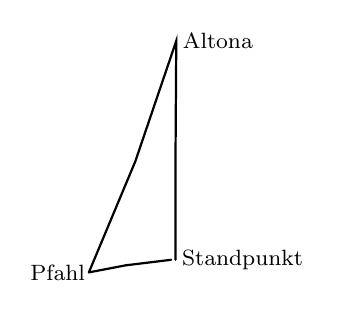
\begin{tikzpicture}[x=1mm,y=1mm,line width=.8pt,line cap=round]
  \coordinate (Pfahl) at (0,0);
  \coordinate (Altona) at (11.1,29.4);
  \coordinate (Standpunkt) at (11.0,1.6);
  \draw (Pfahl) -- (5.9,14.1) -- (Altona) -- (11.0,14.0) -- (Standpunkt);
  \draw (Pfahl) -- (4.7,.9) -- (10.45,1.6);
  \node[font=\footnotesize,anchor=east,inner sep=1pt] at (Pfahl) {Pfahl};
  \node[font=\footnotesize,anchor=west,inner sep=2pt] at (Altona) {Altona};
  \node[font=\footnotesize,anchor=west,inner sep=2pt] at (Standpunkt) {Standpunkt};
 \end{tikzpicture}
\end{minipage}\hfill
\begin{minipage}[t]{.71\linewidth}
 \vspace{0pt}
 \setlength{\parindent}{1.5em}
 \indent I,\quad Den Winkel in Altona zwischen den Richtungen zum Pfahl und zum Standpunkt.

 II.\quad Eine kleine Korrektur wegen der Erdkrümmung, durch die der Unterschied zwischen den Richtungen Altona-Standpunkt und Standpunkt-Altona geringfügig von \(180^\circ\) abweicht. Beide Berichtigungen können
\end{minipage}\par
\noindent aber erst berechnet werden, wenn die Lage des Standpunkts wenigstens näherungsweise bekannt ist. Man kann diese also zuerst suchen und die beiden Berichtigungen vorerst außer Betracht lassen. Dazu braucht es keine Anleitung. Sie können nach Belieben das \(\Delta\) Altona, Standpunkt, Hamburg oder Altona, Standpunkt, Rönneberg usw. dazu verwenden. Ich bemerke nur, dass zur Berechnung von I. lediglich die Entfernung Altona-Standpunkt nötig ist. Im obigen Dreieck sind dann 2 Seiten und ein Winkel bekannt. Ich finde nun
\[
\raisebox{\baselineskip}{\(\displaystyle
\GaussRightBrace{
\begin{array}{@{}l@{\;=\;}l@{}}
 \log(\text{Altona-Standpunkt})&4{,}09915\\
 \log(\text{Standpunkt-Pfahl})&0{,}16643\\
 \text{Winkel [am] Standpunkt}&129^\circ36'58''
\end{array}}
\)}
\begin{array}{@{}l@{\;}c@{\;}r@{}}
 \text{Der Winkel in Altona}&=&18''{,}551\\
 \text{und somit, da in Altona}&&\\
 \text{Azimut des Pfahls}&=&13^\circ\,34'\,20''{,}225,\\
 \cline{2-3}
 \text{ebendort}&&\\
 \text{Azimut des Standpunkts}&=&13^\circ\,34'\,1''{,}674.
\end{array}
\]

Zu II. bemerke ich, dass für diese Korrektur die angenäherten Koordinaten des Standpunkts nötig sind.

Sind die Koordinaten von Altona \(a,b\),\par
die des Standpunkts \(x,y\),\par
so ist die Korrektur \(=-A(x-a)(y+b)\),\par
\noindent wobei \(A\) eine Größe ist, die eigentlich eine Funktion von \(x\), genauer von \(\frac12(x+a)\), ist, sich aber sehr langsam ändert[*)].
\[
\begin{array}{@{}c@{\quad}l@{\quad}c@{\enspace}c@{\;=\;}l@{}}
 \text{Für}&\text{Altona}&\text{ist}&\log A&1{,}40336-10\\
 \text{»}&\text{Lysabbel}&\text{»}&\text{»}&1{,}40323-10.
\end{array}
\]
\indent Die Rechnung sieht also folgendermaßen aus.
\[
\begin{array}{@{}r@{\;=\;}r@{\qquad}r@{\;=\;}r@{\enspace}l@{}}
 a&-224495{,}3&b&+16{,}4&\\
 x&-212281{,}4&y&+2963{,}7&\text{(sind übrigens schon gute Koordinaten)}
\end{array}
\]

\par\smallskip\noindent\rule{4cm}{.4pt}\par
{\footnotesize\noindent\hspace*{\parindent}[*) Vgl. S.~216/217, wo \(q\) für \(A\) geschrieben ist. Nimmt man \(A\) für beide Punkte als gleich an, so ist die Korrektur \(-A(x-a)\dfrac{2b+y}{3}+A(a-x)\dfrac{2y+b}{3}\).]\par}

% Printed 287; principal PDF 294; Google PDF 298.
\par\clearpage
\noindent\null\hfill{\small\textbf{STATIONSAUSGLEICHUNGEN.}}\hfill\makebox[0pt][r]{\fontsize{13}{16}\selectfont 287}\par\medskip

\[
\begin{array}{@{}r@{\;=\;}r@{\qquad}l@{\enspace}l@{}}
 x-a&+12213{,}9&\log.\,.\,.\,.\,.\,.&4{,}08686\\
 y+b&+2980{,}1&\log.\,.\,.\,.\,.\,.&3{,}47423\\
 \multicolumn{2}{c}{}&\log(-A).\, .&1{,}40336_n-10\\
 \cline{3-4}
 \multicolumn{2}{c}{}&&8{,}96445_n-10.
\end{array}
\]
\[
\begin{array}{@{}r@{\quad}c@{\;}l@{}}
 \text{Zahl}&=&\qquad-0''{,}092.\\[3pt]
 \text{Azimut \textls[120]{in} Altona}&=&13^\circ\,34'\,1''{,}674\\
 &&180\\
 \cline{3-3}
 \text{Azimut \textls[120]{von} Altona}&=&193^\circ\,34'\,1''{,}582.
\end{array}
\]
\indent Die obige Tabelle benötigt zur Orientierung also eine Korrektur von \(-28''{,}394\) und sieht damit folgendermaßen aus.
\[
\begin{array}{@{}l@{\enspace}r@{\;}r@{\;}l@{}}
 \text{\hbox to 8.7em{Pfahl\hfil.\hfil.\hfil.\hfil.\hfil.\hfil.\hfil.\hfil.\hfil.}}&63^\circ&57'&4''\\
 \text{\hbox to 8.7em{Neuenfelde\hfil.\hfil.\hfil.\hfil.}}&148&22&31{,}267\\
 \text{\hbox to 8.7em{Altenwerder\hfil.\hfil.\hfil.}}&189&27&10{,}451\\
 \multicolumn{4}{c}{\text{usw.}}
\end{array}
\]

\begin{center}\rule{3cm}{.4pt}\end{center}
\vspace{.8cm}
\begingroup\small
\begin{center}
 BEMERKUNGEN.
\end{center}

Eine Zusammenstellung der endgültigen Ausgleichungen von Stationsbeobachtungen, deren Ergebnisse in die Netzausgleichung eingeführt wurden, liegt nicht vor. Die Ergebnisse der Stationsausgleichungen selbst sind in Band IV, S.~449 ff., in den »Abrissen der auf den verschiedenen Stationen der Gradmessung, 1821, 1822, 1823, und deren Fortsetzung bis Jever, 1824, 1825, festgelegten Richtungen.« mitgeteilt. Doch weichen die Richtungswerte, die \textsc{Gauss} für die Netzausgleichung verwendet hat, noch geringfügig von jenen ab, wie aus der Zusammenstellung der beobachteten Winkel nach Dreiecken im folgenden Abschnitt hervorgeht. Die Abweichungen ergeben sich aus den Reduktionen wegen der Höhe des anvisierten Objekts und wegen der Abweichung der geodätischen Linie vom Vertikalschnitt (vgl. dazu den weiter unten wiedergegebenen Brief an \textsc{Olbers} vom 14. Mai 1826). Bei manchen Richtungen müssen sie aber auch auf Zentrierungsbeträge zurückgehen.

Die hier mitgeteilten Stationsausgleichungen für Zeven und Brillit, [1] und [2], sind vorläufig und stammen aus einem Notizbuch, in das \textsc{Gauss} insgesamt 8 Ausgleichungen von Stationsbeobachtungen eingetragen hatte. Anstelle der angegebenen Konstanten in der dritten und vierten Normalgleichung für Zeven hatte \textsc{Gauss} irrtümlich \(+0{,}346\) und \(-1{,}189\). Infolgedessen weicht seine Lösungstabelle von der oben angegebenen ab. Je nach Stand der Beobachtungen hat \textsc{Gauss} die Ausgleichungen mehrmals wiederholt (vgl. S.~280, unten). So ist die hier mitgeteilte Ausgleichung für die Station Wilsede, Notiz [3], die vierte. Sie stand in einem Beobachtungs- und Rechnungsheft für die hannoversche Gradmessung. Ihr Ergebnis stimmt mit der Angabe in den »Abrissen

% Printed 288; principal PDF 295; Google PDF 299.
\par\clearpage
\noindent\makebox[0pt][l]{\fontsize{13}{16}\selectfont 288}\hfill{\small\textbf{BEMERKUNGEN.}}\hfill\null\par\medskip

\noindent etc.«, Band IV, S.~454, überein, wenn man hier die Orientierung um \(-0''{,}665\) ändert. Berechnet man nach Art.~13, S.~95, für Wilsede die Korrekturen der beobachteten Richtungen wegen der Höhe des anvisierten Objekts über dem Meeresspiegel und wegen der Abweichung der geodätischen Linie vom Vertikalschnitt, so erhält man für die Richtung nach Falkenberg (150,8 m) \(+0''{,}001\), nach Elmhorst (90,0 m) \(+0''{,}003\), für die Richtungen nach Steinberg (72,3 m), Bottel (52,4 m), Bullerberg (53,3 m), Brüttendorf (49,6 m) und Zeven (44,8 m) je \(0''{,}000\), für die Richtung nach Litberg (65,5 m) \(-0''{,}001\), nach Hamburg (144,9 m) \(0''{,}000\), nach Lüneburg (99,1 m) \(+0''{,}002\), nach Nindorf (116,7 m) \(-0''{,}001\), nach Timpenberg (117,1 m) \(-0''{,}002\), nach Wulfsode (104,5 m) \(-0''{,}003\), nach Breithorn (120,5 m) \(-0''{,}002\) und nach Hauselberg (120,4 m) \(-0''{,}002\). Die in Klammern angegebenen Höhen über dem Meeresspiegel stammen aus einem Notizbuch von \textsc{Gauss}. Bringt man diese Korrekturen an den Ausgleichungsergebnissen an, so ergeben sich die für Wilsede in die Netzausgleichung eingeführten Werte.

Sämtliche noch vorhandenen Stationsausgleichungen finden sich teils in kleinen Beobachtungs- und Rechnungsheften zur Gradmessung, teils verstreut auf losen Blättern. Die Form der Ausgleichung ist bei allen Hauptdreieckspunkten wie bei Zeven oder Wilsede, in wenigen Fällen wie bei Brillit (vgl. die Briefe an \textsc{Olbers} vom Juli 1825, an \textsc{Schumacher} vom 14. August 1825 und an \textsc{Bessel} vom 29. Oktober 1843).

Die Messungen wurden auf keinem Hauptdreieckspunkt symmetrisch angeordnet. Nur auf einigen Nebenpunkten scheinen alle Winkelkombinationen beobachtet worden zu sein. Ein Beispiel dafür geben die Beobachtungen auf dem Windberg, Notiz [4], des Artillerieleutnants F.~\textsc{Hartmann}, eines Gehilfen von \textsc{Gauss} bei der Triangulation. (Auf dem Original, einem einzelnen Blatt, hat \textsc{Hartmann} noch hinzugefügt: »Wegen Abgang der Post nicht vollständig. Den Winkel \(7.3\) will ich noch einmal messen, vielleicht hat diese Wiederholung auch auf den Winkel \(3.5\) einen günstigen Einfluss«. Nach dem Beobachtungsbuch ist sie aber nicht erfolgt.) Die Messungen auf dem Windberg fanden im Juni 1830 statt.

Wie \textsc{Gauss} beobachtet hat, zeigt der Auszug aus einem Beobachtungsheft für den Gradmessungspunkt Breithorn, Notiz [5].

Über das bei der hannoverschen Triangulation angewandte Verfahren gibt auch der folgende Auszug aus dem bereits erwähnten Heftchen »Geodätischer Calcül nach \textsc{Gauss}« von Prof. \textsc{Goldschmidt} Auskunft. Wie bereits erwähnt, hat \textsc{Goldschmidt} \textsc{Gauss} wahrscheinlich in den letzten Jahren der Landesvermessung bei den Rechnungen unterstützt. 1834 nahm er bei Leutnant \textsc{Gauss} an den Messungen für die Detailaufnahme teil.

»Bei der Triangulation selbst wählt man zuerst eine mäßige Anzahl von Punkten aus, die das aufzunehmende Gebiet so abdecken, dass sie eine weite Aussicht bieten. Von diesen \textls[120]{Hauptpunkten} wählt man nur so viele aus, wie zur Bestimmung der sogenannten Punkte zweiter Ordnung nötig sind, von denen gleich die Rede sein wird. Im Übrigen wählt man ihren Abstand so groß, wie das Gelände und die Stärke der verwendeten Fernrohre es zulassen. Auf \textls[120]{jedem} der ausgewählten Hauptdreieckspunkte schneidet man alle sichtbaren Objekte ein, die bestimmt werden sollen. Man misst aber hauptsächlich die Winkel zwischen den übrigen von dort sichtbaren Hauptpunkten mit vielfacher Repetition und ebenso die Winkel zwischen den ausgewählten Nebenpunkten und den Hauptpunkten.

Die Hauptdreieckspunkte dienen dazu, dem ganzen System Halt zu geben. Deshalb wählt man nur wenige von ihnen und setzt ihren Abstand möglichst groß an, um weniger Zwischenstationen zu haben, an denen sich die gemachten Fehler immer weiter anhäufen könnten.

Die geringe Zahl der ausgewählten Hauptdreieckspunkte würde es uns aber unmöglich machen, alle von ihnen umschlossenen Punkte genau zu bestimmen, selbst wenn das Gelände es erlaubte,

% Printed 289; principal PDF 296; Google PDF 300.
\par\clearpage
\noindent\null\hfill{\small\textbf{STATIONSAUSGLEICHUNGEN.}}\hfill\makebox[0pt][r]{\fontsize{13}{16}\selectfont 289}\par\medskip

\noindent alle festzulegenden Punkte anzuvisieren. Denn dabei ließe es sich nicht vermeiden, dass viele Punkte durch sehr spitze Dreiecke bestimmt werden müssten, in denen bekanntlich ein sehr kleiner Fehler bei der Winkelmessung die Lage des Punktes erheblich verändern würde. Aus diesem Grund wählt man noch eine größere Anzahl von \textls[120]{Nebenpunkten} aus.

Diese wählt man so, dass sie 1) zur Bestimmung \textls[120]{aller} festzulegenden Punkte genügen und 2) sich \textls[120]{nach Möglichkeit} von den Hauptdreieckspunkten aus mit \textls[120]{Genauigkeit} bestimmen lassen. Dabei braucht man allerdings nicht zu streng zu sein. Lässt sich ein solcher Punkt nicht von Hauptdreieckspunkten aus bestimmen, so kann man ihn von Nebenpunkten aus bestimmen. Der Orientierung halber ist es jedoch immer gut, wenigstens einen Hauptdreieckspunkt einzuschneiden. Auch von den Nebenpunkten aus schneidet man \textls[120]{alle sichtbaren} Objekte ein, die bestimmt werden sollen, die Haupt- und Nebenpunkte mit mehrfacher Repetition und Ablesung, die übrigen Punkte, die keine Standpunkte sind, notfalls nur einmal.

Das ist die allgemeine Übersicht über die Triangulation. Nun folgen einige Bemerkungen zu den Einzelheiten.\par
\noindent Beim Drehen des Alhidadenkreises dreht sich der Teilkreis stets etwas mit, wenn auch nur geringfügig. Dadurch können konstante Fehler entstehen, sodass man beim Messen von links nach rechts die Winkel immer zu klein finden würde, wenn man den Alhidadenkreis stets auf dem kürzesten Weg zum Objekt bewegt. (Bei der Auswertung der Messungen, die Leutnant \textsc{Gauss} 1833 in Westfalen vorgenommen hat, fand ich den daraus entstehenden mittleren Fehler zu etwa \(1''{,}5\), bei den Messungen von Hauptmann \textsc{Müller} zu \(3''\).) Um dies auszugleichen, führt \textsc{Gauss} den Alhidadenkreis ebenso oft auf dem kürzesten wie auf dem längsten Weg in die Richtung des zweiten Objekts.

\begin{center}
 \textls[120]{Messung der Winkel von einem Standpunkt aus.}
\end{center}

Wir wählen zuerst einige Punkte aus, deren Gestalt ein genaues Anvisieren ermöglicht. Für genaue Ergebnisse sollten es wohl mindestens 4 sein, und zur Vermeidung unnötigen Aufwands höchstens 6. Am besten sind es Hauptpunkte des Systems, die zugleich den Horizont in gleiche Teile teilen. Diese Bedingungen braucht man jedoch nicht allzu streng zu nehmen. Man misst nun die Winkel zwischen je zwei dieser Objekte und bildet dabei alle möglichen Kombinationen. Danach gleicht man die gefundenen Werte nach der Methode der kleinsten Quadrate aus. Jeden anderen festzulegenden Punkt vergleichen wir nun mit einer der so bestimmten Richtungen. Soll er genauer bestimmt werden, so geschieht dies durch mehrfache Repetition. Vielleicht vergleichen wir ihn auch mit zwei Richtungen. Liefern diese nicht dasselbe Ergebnis, so wendet man auch hier die Methode der kleinsten Quadrate an. Wie das geschieht, geben wir sogleich an.

Wir zeigen die Anwendung der Methode der kleinsten Quadrate an einem Beispiel. Vom Standpunkt \textls[120]{Hoheegge} aus wurden \textls[120]{Enegerloh} (1), \textls[120]{Dörenberg} (2), \textls[120]{Nonnenstein} (3) und \textls[120]{Hünenburg} (4) als Vergleichspunkte ausgewählt und die folgenden Winkel jeweils mit 20-facher Repetition gemessen.
\[
\begin{array}{@{}r@{\;=\;}r@{\;}r@{\;}l@{}}
 1.2&77^\circ&42'&38''{,}313\\
 1.3&162&40&2{,}500\\
 2.3&84&57&24{,}750\\
 3.4&107&59&41{,}375\\
 4.1&89&20&16{,}438\\
 4.2&167&2&53{,}025.
\end{array}
\]

Man nehme nun die Azimute der 4 Punkte 1, 2, 3, 4, beziehe sie also alle auf ein und dieselbe Grundrichtung. Ob diese wirklich der Meridian ist, spielt dabei keine Rolle, doch ist es ratsam,
\par\smallskip\noindent\makebox[0pt][l]{\small IX.}\makebox[.86\linewidth][r]{37}\par

% Printed 290; principal PDF 297; Google PDF 301.
\par\clearpage
\noindent\makebox[0pt][l]{\fontsize{13}{16}\selectfont 290}\hfill{\small\textbf{BEMERKUNGEN.}}\hfill\null\par\medskip

\noindent diese Richtung nahe am Meridian zu wählen, damit die spätere Korrektur für die Orientierung nicht zu groß ausfällt. Die ungefähre Richtung des Meridians lässt sich nötigenfalls immer mit der Bussole bestimmen (wie \textsc{Hartmann} es im Harz tat, wo er kein Azimut kannte). Ein Näherungswert des Azimuts von 1 ist \(41^\circ25'0''{,}0\). Wären alle Winkel, von denen 1 ein Schenkel ist, richtig gemessen, so wären die Azimute von
\[
\begin{array}{@{}r@{\;=\;}r@{\;}r@{\;}l@{}}
 2&119^\circ&7'&38''{,}313\\
 3&204&5&2{,}500\\
 4&312&4&43{,}562.
\end{array}
\]

Berechnet man beispielsweise 3 statt aus 1 und \(1.3\) aus 2 und \(2.3\), so findet man \(3=2+2.3=204^\circ5'3''{,}063\), was vom oben angegebenen Wert abweicht. Für 2, 3, 4 sind also noch Korrekturen nötig. Die Werte für 2, 3, 4 sind nur angenähert. Zur Vereinfachung der Rechnung lassen wir die Dezimalteile der Bogensekunde weg und beziehen sie in die Korrektur ein. Damit ergibt sich
\[
\begin{array}{@{}r@{\;=\;}r@{\;}r@{\;}r@{\;}l@{}}
 1&41^\circ&25'&0''{,}0&\\
 2&119&7&38{,}0&+x\\
 3&204&5&2{,}0&+y\\
 4&312&4&43{,}0&+z.
\end{array}
\]

Berechnet man daraus die Winkel, so ergibt sich Folgendes.
\[
\begin{array}{@{}r@{\;=\;}r@{\;}r@{\;}r@{\;}l|r|r@{\;}l@{\;=\;}l@{}}
 \multicolumn{5}{c}{\text{Ber.}}&
 \multicolumn{1}{c}{\text{Beob.}}&
 \multicolumn{3}{c}{\text{Beob.-Ber.}}\\
 1.2&77^\circ&42'&38''{,}0&+x&38''{,}313&-0''{,}313&+x&\varepsilon'\\
 1.3&162&40&2{,}0&+y&2{,}500&-0{,}500&+y&\varepsilon''\\
 2.3&84&57&24{,}0&-x+y&24{,}750&-0{,}750&-x+y&\varepsilon'''\\
 3.4&107&59&41{,}0&-y+z&41{,}375&-0{,}375&-y+z&\varepsilon^{\mathrm{IV}}\\
 4.1&89&20&17{,}0&-z&16{,}438&+0{,}562&-z&\varepsilon^{\mathrm{V}}\\
 4.2&167&2&55{,}0&+x-z&53{,}025&+1{,}975&+x-z&\varepsilon^{\mathrm{VI}}
\end{array}
\raisebox{-.5\baselineskip}{%
 \(\GaussRightBrace{\vphantom{\begin{array}{c}0\\0\\0\\0\\0\\0\end{array}}}\)%
 \enspace\rotatebox[origin=c]{-90}{Fehlergleichungen.}%
}
\]

Bildet man daraus nach der Methode der kleinsten Quadrate die Grundgleichungen, so erhält man
\[
\begin{array}{@{}r@{\;}r@{\;}r@{\;}r@{\;=\;}l@{}}
 +2{,}412&+3x&-y&-z&0\\
 -0{,}875&-x&+3y&-z&0\\
 -2{,}912&-x&-y&+3z&0.
\end{array}
\]

Gleichungen dieser Form lassen sich am besten folgendermaßen lösen. Addiert man sie, so erhält man
\[
 -1{,}375+x+y+z=0,
\]
und durch Addition dieser Gleichung zu jeder einzelnen Grundgleichung erhält man Folgendes.
\[
\begin{array}{@{}r@{\;}l@{\;=\;}r@{\qquad}c@{\;=\;}l@{}}
 +1{,}037&+4x&0&x&-0{,}259\\
 -2{,}250&+4y&0&y&+0{,}563\\
 -4{,}287&+4z&0&z&+1{,}072.
\end{array}
\]

Dieses einfache Eliminationsverfahren lässt sich stets auf die symmetrischen Grundgleichungen anwenden, zu denen diese Aufgabe führt, wenn alle Kombinationen der Richtungen mit gleich vielen Repetitionen gemessen wurden. Wir erhalten also die verbesserten Azimute.

% Printed 291; principal PDF 298; Google PDF 302.
\par\clearpage
\noindent\null\hfill{\small\textbf{STATIONSAUSGLEICHUNGEN.}}\hfill\makebox[0pt][r]{\fontsize{13}{16}\selectfont 291}\par\medskip

\[
\begin{array}{@{}l@{\quad}r@{\;}r@{\;}r@{\quad}l@{\quad}r@{\quad}r@{\;}r@{\;}r|l@{}}
 \multicolumn{6}{c}{}&\multicolumn{3}{c}{\text{Ber.}}&\multicolumn{1}{c}{\text{Ber.-Beob.}}\\
 1.&41^\circ&25'&0''{,}000&&1.2&77^\circ&42'&37''{,}741&-0''{,}572\\
 2.&119&7&37{,}741&&1.3&162&40&2{,}563&+0{,}063\\
 3.&204&5&2{,}563&&2.3&84&57&24{,}822&+0{,}072\\
 4.&312&4&44{,}072&\text{und daraus}&3.4&107&59&41{,}509&+0{,}134\\
 &&&&&4.1&89&20&15{,}928&-0{,}510\\
 &&&&&4.2&167&2&53{,}669&+0{,}644.
\end{array}
\]

Sind die Winkel mit unterschiedlicher Anzahl von Repetitionen gemessen und haben daher verschiedene Gewichte, so muss man jeden Beitrag der Fehlergleichungen für \(\varepsilon',\varepsilon'',\varepsilon''',\ldots\) zu den Grundgleichungen mit dem jeweiligen Gewicht multiplizieren, also mit der Zahl, die der Anzahl der Repetitionen proportional ist. Als Beispiel dafür nehmen wir die von [Leutnant] \textsc{Gauss} in \textls[120]{Neuenkirchen} gemessenen Winkel.

\begin{center}
 1. Dörenberg\qquad 2. Quekenberg\qquad 3. Quackenbrück\qquad 4. Mordkuhlenberg.
\end{center}

Er fand
\[
\begin{array}{@{}r@{\quad}r@{\;}r@{\;}r@{\quad}c@{\qquad}l@{\quad}r@{\;}r@{\;}r@{\;}l@{}}
 \multicolumn{4}{c}{}&\text{Gew.}&
 \multicolumn{5}{c}{\text{Azimute}}\\
 1.2&93^\circ&9'&2''{,}875&5&1.&6^\circ&25'&58''{,}000&\quad\text{[*)]}\\
 1.3&147&10&10{,}938&1&2.&99&35&0{,}875&+b\\
 2.3&54&1&4{,}125&5&3.&153&36&5{,}656&+c\\
 3.4&86&21&14{,}875&5&4.&239&57&22{,}453&+d\\
 4.1&126&28&33{,}625&5&&&&&\\[3pt]
 &\multicolumn{3}{c}{\text{Ber.-Beob.}}&\text{Gew.}&&&&&\\
 1.2&&&0''{,}000+b&5&&&&&\\
 1.3&&&-3{,}282+c&1&&&&&\\
 2.3&&&+0{,}656-b+c&5&&&&&\\
 3.4&&&+1{,}922-c+d&5&&&&&\\
 4.1&&&+1{,}922-d&5.&&&&&
\end{array}
\]

Bildet man die Grundgleichungen, indem man die Beiträge der obigen Fehlergleichungen mit ihren jeweiligen Gewichten multipliziert, so erhält man
\[
\begin{array}{@{}r@{\;}c@{\;}r@{\;}c@{\;=\;}l@{}}
 -3{,}280&+10b&-5c&*&0\\
 -9{,}612&-5b&+11c&-5d&0\\
 \multicolumn{1}{c@{\;}}{0}&*&-5c&+10d&0,
\end{array}
\]
und nun bestimmt man \(b,c,d\) nach den bekannten Regeln und verbessert damit die obigen Azimutwerte.

Hat man auf diese Weise die zwischen den Hauptrichtungen gemessenen Winkel ausgeglichen, so bestimmt man damit die übrigen Richtungen, die, wie schon gesagt, beim Einschneiden mit einer der gewählten Hauptrichtungen verbunden werden. Ist zum Beispiel ein Punkt \(A\) mit der Hauptrichtung 1, deren Azimut wir 1 nennen, dadurch verbunden, dass der Winkel \(1.A\) gemessen wurde, so ergibt sich das Azimut von \(A=1+1.A\).

\par\smallskip\noindent\rule{4cm}{.4pt}\par
{\footnotesize\noindent\hspace*{\parindent}[*) In einem Vorlesungsheft über höhere Geodäsie, das auch dieses Beispiel enthält, wird der Richtung nach 1 ebenfalls eine Verbesserung zugewiesen, sodass die Summe der Normalgleichungen null wird.]\par}
\par\smallskip\noindent\makebox[.86\linewidth][r]{37\textsuperscript{*}}\par
\endgroup
